\documentclass[aspectratio=169,10pt]{beamer}

\usetheme{metropolis}
\usecolortheme{default}

\usepackage[T1]{fontenc}
\usepackage[utf8]{inputenc}
\usepackage{booktabs}
\usepackage{amsmath,amssymb}
\usepackage{graphicx}
\usepackage{xcolor}
\usepackage{tikz}
\usetikzlibrary{positioning,arrows.meta}
\usepackage{array}

\definecolor{luhblue}{RGB}{21,101,192}
\definecolor{alertred}{RGB}{198,40,40}
\definecolor{okgreen}{RGB}{27,94,32}

\setbeamercolor{frametitle}{bg=luhblue, fg=white}
\setbeamercolor{progress bar}{fg=luhblue}
\setbeamercolor{alerted text}{fg=alertred}
\setbeamercolor{example text}{fg=okgreen}
\metroset{progressbar=frametitle, block=fill}

% Institution logos top-right on every frame (graceful if files absent).
% Drop the OFFICIAL files into slides/ to show them (request usage rights first):
%   keio-logo.{pdf,png}  luh-logo.{pdf,png}  jaxa-logo.{pdf,png}
\newcommand{\maybelogo}[1]{%
  \IfFileExists{#1.pdf}{\includegraphics[height=6mm]{#1}\hspace{2mm}}{%
    \IfFileExists{#1.png}{\includegraphics[height=6mm]{#1}\hspace{2mm}}{}}}
\addtobeamertemplate{frametitle}{}{%
  \begin{tikzpicture}[remember picture, overlay]
    \node[anchor=north east, xshift=-3mm, yshift=-1.2mm] at (current page.north east){%
      \maybelogo{keio-logo}\maybelogo{luh-logo}\maybelogo{jaxa-logo}%
    };
  \end{tikzpicture}%
}

\title{From Defect Detection to Flight Clearance:\\
a Bayesian SHM Stack for Reusable Launch Vehicles}
\subtitle{Stage 0--3 implemented and verified on CFRP thermoelastic fields}
\author{Keisuke Nishioka}
\institute{Leibniz Universit\"at Hannover \quad$\cdot$\quad Keio University}
\date{June 2026}

\begin{document}
\maketitle

% ─────────────────────────────────────────────
\begin{frame}{Motivation: reusable rockets change the question}
\begin{columns}[T]
\column{0.55\textwidth}
\textbf{Expendable:} ``will it survive one flight?''\\[2mm]
\textbf{Reusable:} \alert{``is this vehicle OK to fly \emph{again} --- and how many flights remain?''}
\begin{itemize}
  \item Same vehicle re-inspected after every flight\\
        $\Rightarrow$ \emph{fixed geometry, fixed individual} is the norm
  \item SpaceX (empirically): condition-based monitoring, staged certification
        $20 \rightarrow 40$ flights, fleet-leader strategy (B1067: 35 flights, 06/2026)
\end{itemize}
\column{0.42\textwidth}
\begin{block}{This work}
Formalise that practice as a measurable, Bayesian, physics-based pipeline ---
applicable from the \emph{first} article.
\end{block}
\end{columns}
\end{frame}

% ─────────────────────────────────────────────
\begin{frame}{The Stage 0--5 stack}
\centering
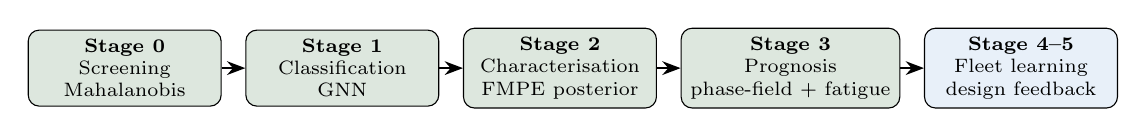
\begin{tikzpicture}[
  box/.style={draw, rounded corners, fill=luhblue!10, minimum width=2.45cm,
              minimum height=9mm, align=center, font=\scriptsize},
  done/.style={box, fill=okgreen!15},
  arr/.style={-{Stealth}, thick}]
\node[done] (s0) {\textbf{Stage 0}\\ Screening\\ Mahalanobis};
\node[done, right=3mm of s0] (s1) {\textbf{Stage 1}\\ Classification\\ GNN};
\node[done, right=3mm of s1] (s2) {\textbf{Stage 2}\\ Characterisation\\ FMPE posterior};
\node[done, right=3mm of s2] (s3) {\textbf{Stage 3}\\ Prognosis\\ phase-field + fatigue};
\node[box, right=3mm of s3] (s4) {\textbf{Stage 4--5}\\ Fleet learning\\ design feedback};
\draw[arr] (s0) -- (s1);
\draw[arr] (s1) -- (s2);
\draw[arr] (s2) -- (s3);
\draw[arr] (s3) -- (s4);
\end{tikzpicture}\\[4mm]
\begin{itemize}
  \item \textcolor{okgreen}{\textbf{Green = implemented and tested}} (2026-06-11, two repos, all committed)
  \item One data contract end-to-end: posterior $\theta=(c_x, c_y, \text{layer}, \text{size})$
        flows from Stage 2 directly into Stage 3
\end{itemize}
\end{frame}

% ─────────────────────────────────────────────
\begin{frame}{Stage 0 --- a 30-line statistic beats eight learned methods}
\begin{columns}[T]
\column{0.58\textwidth}
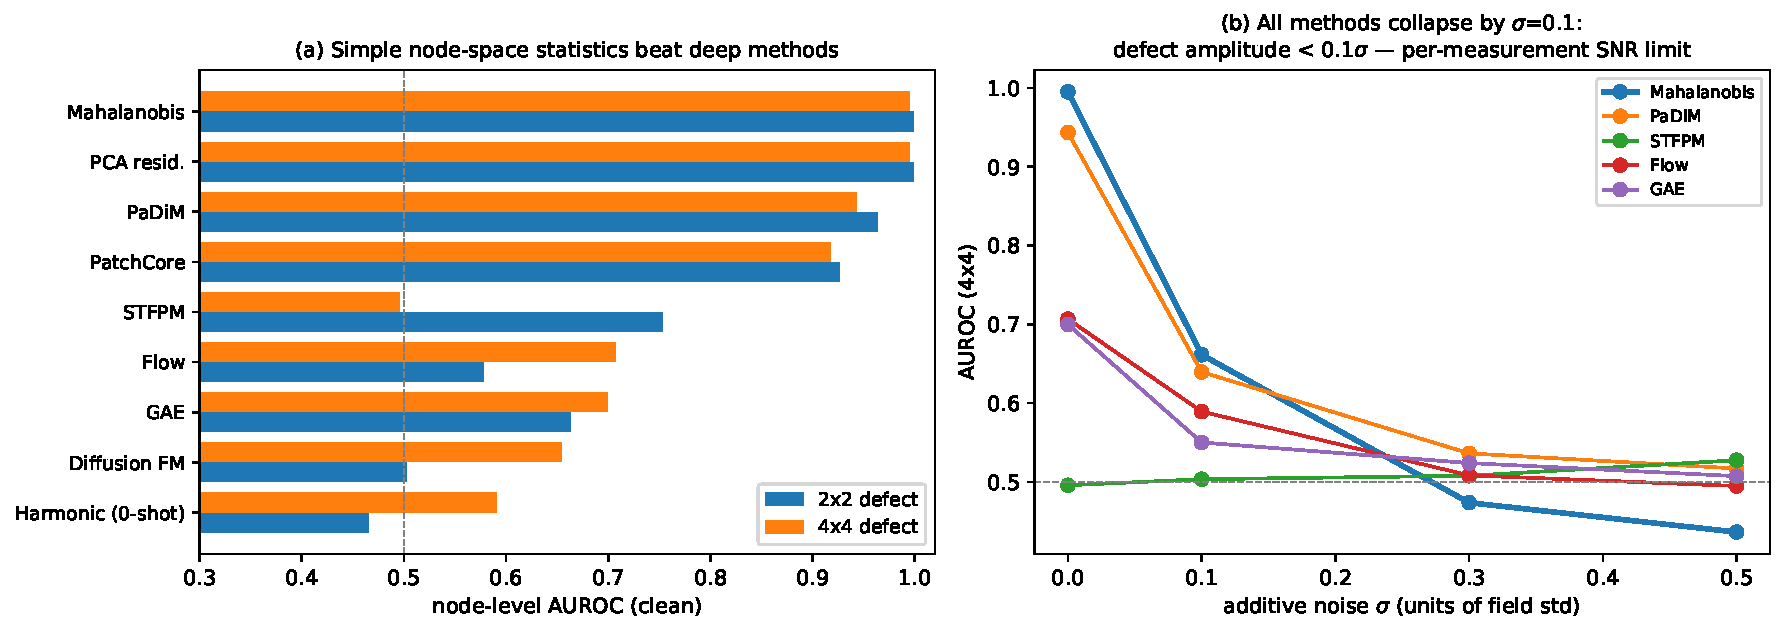
\includegraphics[width=\textwidth]{../paper_figs/anomaly_zoo_benchmark.pdf}
\column{0.40\textwidth}
\textbf{Node-level AUROC (clean):}
\begin{itemize}
  \item per-node Mahalanobis: \textbf{0.999 / 0.995} (2x2/4x4)
  \item deep methods: 0.50--0.75
\end{itemize}
\begin{alertblock}{SNR limit}
All methods collapse at noise $\sigma{=}0.1$:\\ defect amplitude ${<}0.1\sigma$.
Lock-in IR averages $10^3$ cycles $\Rightarrow$ requirement, not blocker.
\end{alertblock}
\end{columns}
\end{frame}

% ─────────────────────────────────────────────
\begin{frame}{Why the simple method wins here --- and why GNN still matters}
\begin{columns}[T]
\column{0.48\textwidth}
\begin{block}{Fixed geometry = template statistics}
Re-inspecting the \emph{same} vehicle: healthy manifold is a point cloud
around one template. Per-node $(\mu_i, \sigma_i)$ is the correct inductive bias.
\end{block}
\column{0.48\textwidth}
\begin{block}{Complementary weaknesses}
\scriptsize
\begin{tabular}{lcc}
\toprule
 & Mahalanobis & GNN \\
\midrule
unknown defect size & \textcolor{okgreen}{open} & \textcolor{alertred}{collapses} \\
noise ($12\%$) & \textcolor{alertred}{dies} & \textcolor{okgreen}{robust} \\
semantic class & --- & \textcolor{okgreen}{only option} \\
new airframe & \textcolor{alertred}{needs refs} & \textcolor{okgreen}{transferable} \\
\bottomrule
\end{tabular}
\end{block}
\end{columns}
\vspace{2mm}
$\Rightarrow$ statistics dominate as a vehicle accumulates flight history;
learned models bootstrap \emph{new} airframes and repairs.
\end{frame}

% ─────────────────────────────────────────────
\begin{frame}{Stage 2 --- calibrated Bayesian defect characterisation (FMPE)}
Flow-matching posterior estimation, trained on the \emph{existing} FEM set
(20k pairs, zero new simulations):
\begin{center}
\begin{tabular}{lccc}
\toprule
parameter & RMSE & $R^2$ & 90\%-coverage \\
\midrule
position $c_x$ & 0.055 & 0.78 & \textbf{0.944} \\
position $c_y$ & 0.021 & 0.83 & \textbf{0.940} \\
size (3-class) & --- & 0.73 (acc.\ 0.82) & 0.894 \\
layer (depth)  & 2.98 & 0.63 & 0.870 \\
\bottomrule
\end{tabular}
\end{center}
\begin{itemize}
  \item Coverage $\approx$ target 0.90 $\Rightarrow$ \textbf{calibrated} posteriors,
        safe to propagate downstream
  \item Depth weakly identifiable --- a physics limit of surface thermoelastic
        measurement, reported honestly
\end{itemize}
\end{frame}

% ─────────────────────────────────────────────
\begin{frame}{Stage 3 --- phase-field prognosis with true fatigue}
\begin{columns}[T]
\column{0.52\textwidth}
\textbf{Model} (12/12 tests green):
\begin{itemize}
  \item multi-ply anisotropic AT2, $A=I+\beta\, a\!\otimes\!a$ per ply
  \item interface bands ($G_c^{int}/G_c^{ply}{=}0.4$, DCB-anchored)
  \item Carrara-2020 fatigue: history $\bar\alpha$ degrades $G_c$
        $\Rightarrow$ W\"ohler-like growth under repeated sub-critical loads
\end{itemize}
\column{0.45\textwidth}
\textbf{Verified physics:}
\begin{itemize}
  \item fiber at $30^\circ$ $\rightarrow$ crack deflects to $23.3^\circ$
  \item low-$G_c$ interface captures crack (73 vs 0 cells)
  \item $P(\text{growth})$ monotone in load: $0 \rightarrow \tfrac23 \rightarrow 1$
\end{itemize}
\end{columns}
\end{frame}

% ─────────────────────────────────────────────
\begin{frame}{Flight clearance --- end-to-end on a real test sample}
Stage 0$\rightarrow$3 run: held-out 4x4 field $\rightarrow$ Mahalanobis map
$\rightarrow$ \emph{trained} FMPE posterior $\rightarrow$ fatigue-aware clearance
(20-flight horizon).
\begin{center}
\begin{tabular}{lccccc}
\toprule
load case & load & fatigue & $P(\text{grow})$ & $\mathbb{E}[\text{flights}]$ & decision \\
\midrule
nominal ascent & 0.06 & \textbf{ON}  & 0.00 & \textbf{19.9} & \textcolor{okgreen}{\textbf{OK}} \\
nominal ascent & 0.06 & off & 0.00 & 11.0 & \textcolor{okgreen}{OK} \\
max-Q gust     & 0.10 & \textbf{ON}  & 1.00 & 0.0  & \textcolor{alertred}{\textbf{RETIRE}} \\
max-Q gust     & 0.10 & off & 0.50 & 1.0  & \textcolor{alertred}{RETIRE} \\
\bottomrule
\end{tabular}
\end{center}
\begin{itemize}
  \item fatigue \emph{accumulates across flights} --- $P(\text{survive }20)$ now
        decays even at constant sub-critical load (no i.i.d.\ shortcut)
  \item thresholds from expected cost (vehicle:repair $=100{:}1 \Rightarrow
        \alpha{=}0.02,\ \beta{=}0.48$)
\end{itemize}
\end{frame}

% ─────────────────────────────────────────────
\begin{frame}{End-to-end, one figure: detect $\rightarrow$ characterise $\rightarrow$ clear}
\centering
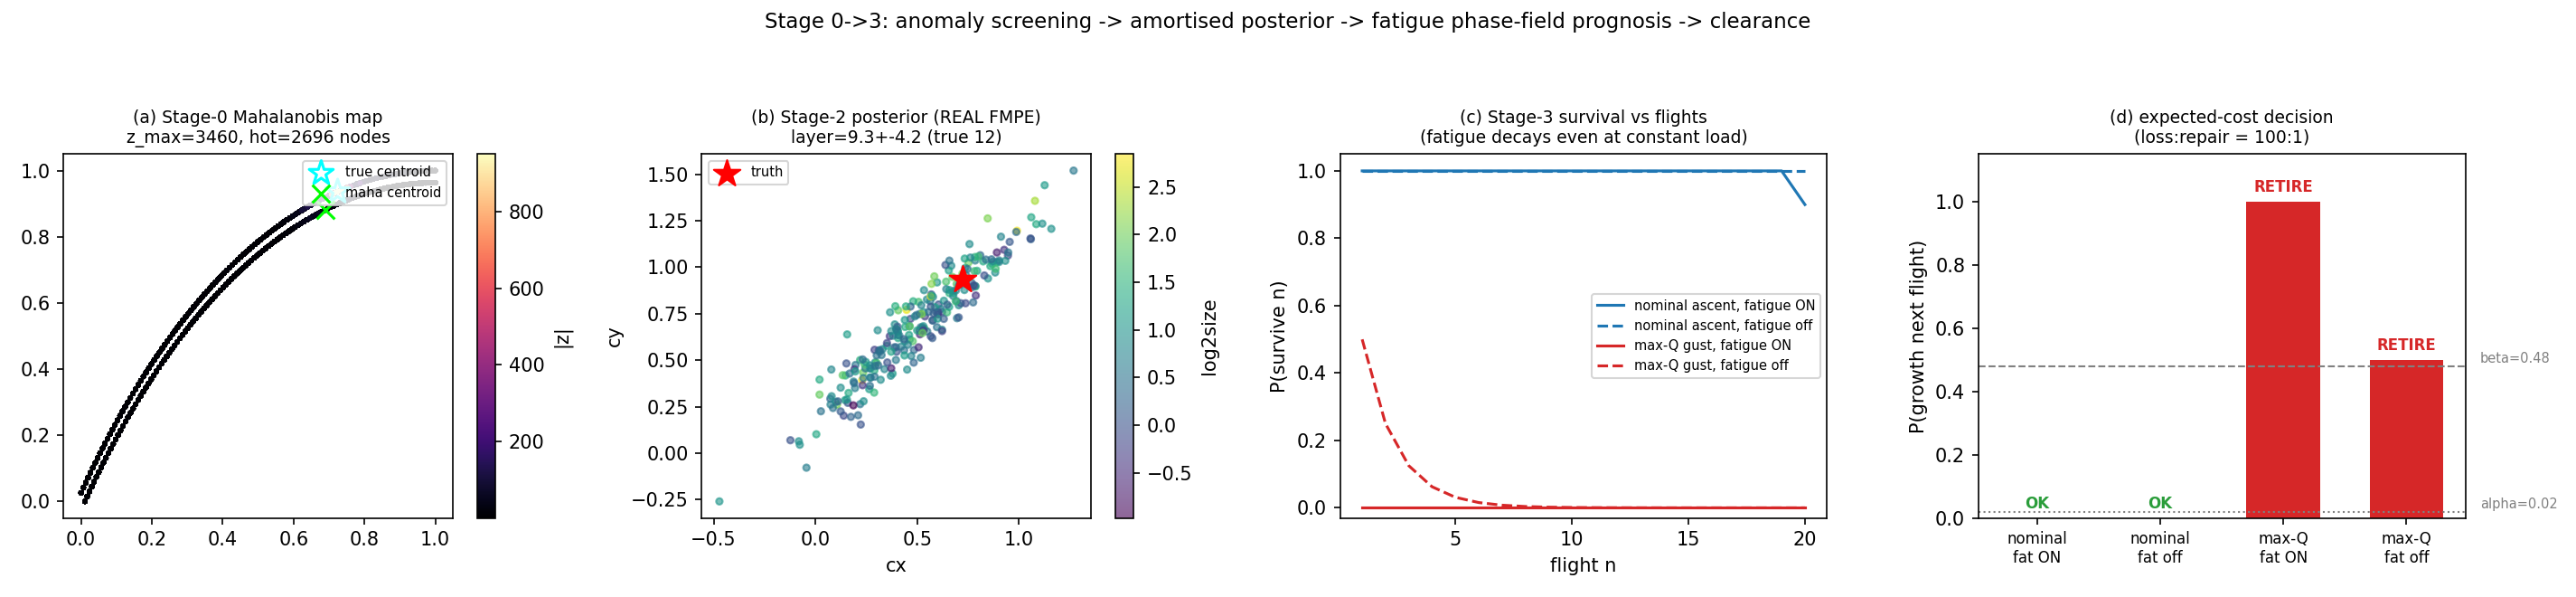
\includegraphics[width=0.92\textwidth]{../results/e2e_stage0to3.png}\\[1mm]
{\scriptsize Stage 0 anomaly map $\cdot$ Stage 2 posterior $\cdot$
$P(\text{survive }n)$ with fatigue $\cdot$ decision --- single held-out CFRP field.}
\end{frame}

% ─────────────────────────────────────────────
\begin{frame}{Outlook: Stage 4--5 and deployment}
\begin{itemize}
  \item \textbf{Stage 4 --- fleet learning:} hierarchical Bayes over tail numbers;
        formalises the SpaceX fleet-leader practice (lead vehicle = likelihood,
        fleet = prior update)
  \item \textbf{Stage 5 --- design feedback:} fleet damage statistics
        $\rightarrow$ layup/reinforcement optimisation (BO)
  \item \textbf{Sim-to-real:} flow-matching bridge ready for first measured
        full-field data (per-sample normalisation needs no healthy reference)
  \item \textbf{Targets:} JAXA reusable-vehicle programmes; journal paper
        (anomaly benchmark + calibrated FMPE + fatigue prognosis)
\end{itemize}
\vspace{2mm}
\begin{block}{One sentence}
SpaceX learned this loop empirically over a decade --- we formalise it so it
works from the first inspection of the first article.
\end{block}
\end{frame}

\end{document}
